\chapter{Implementierung der Liste}
\label{chap:4}

\begin{wrapfigure}{R}{0.5\textwidth}
	\vspace{-\baselineskip}
	\centering
	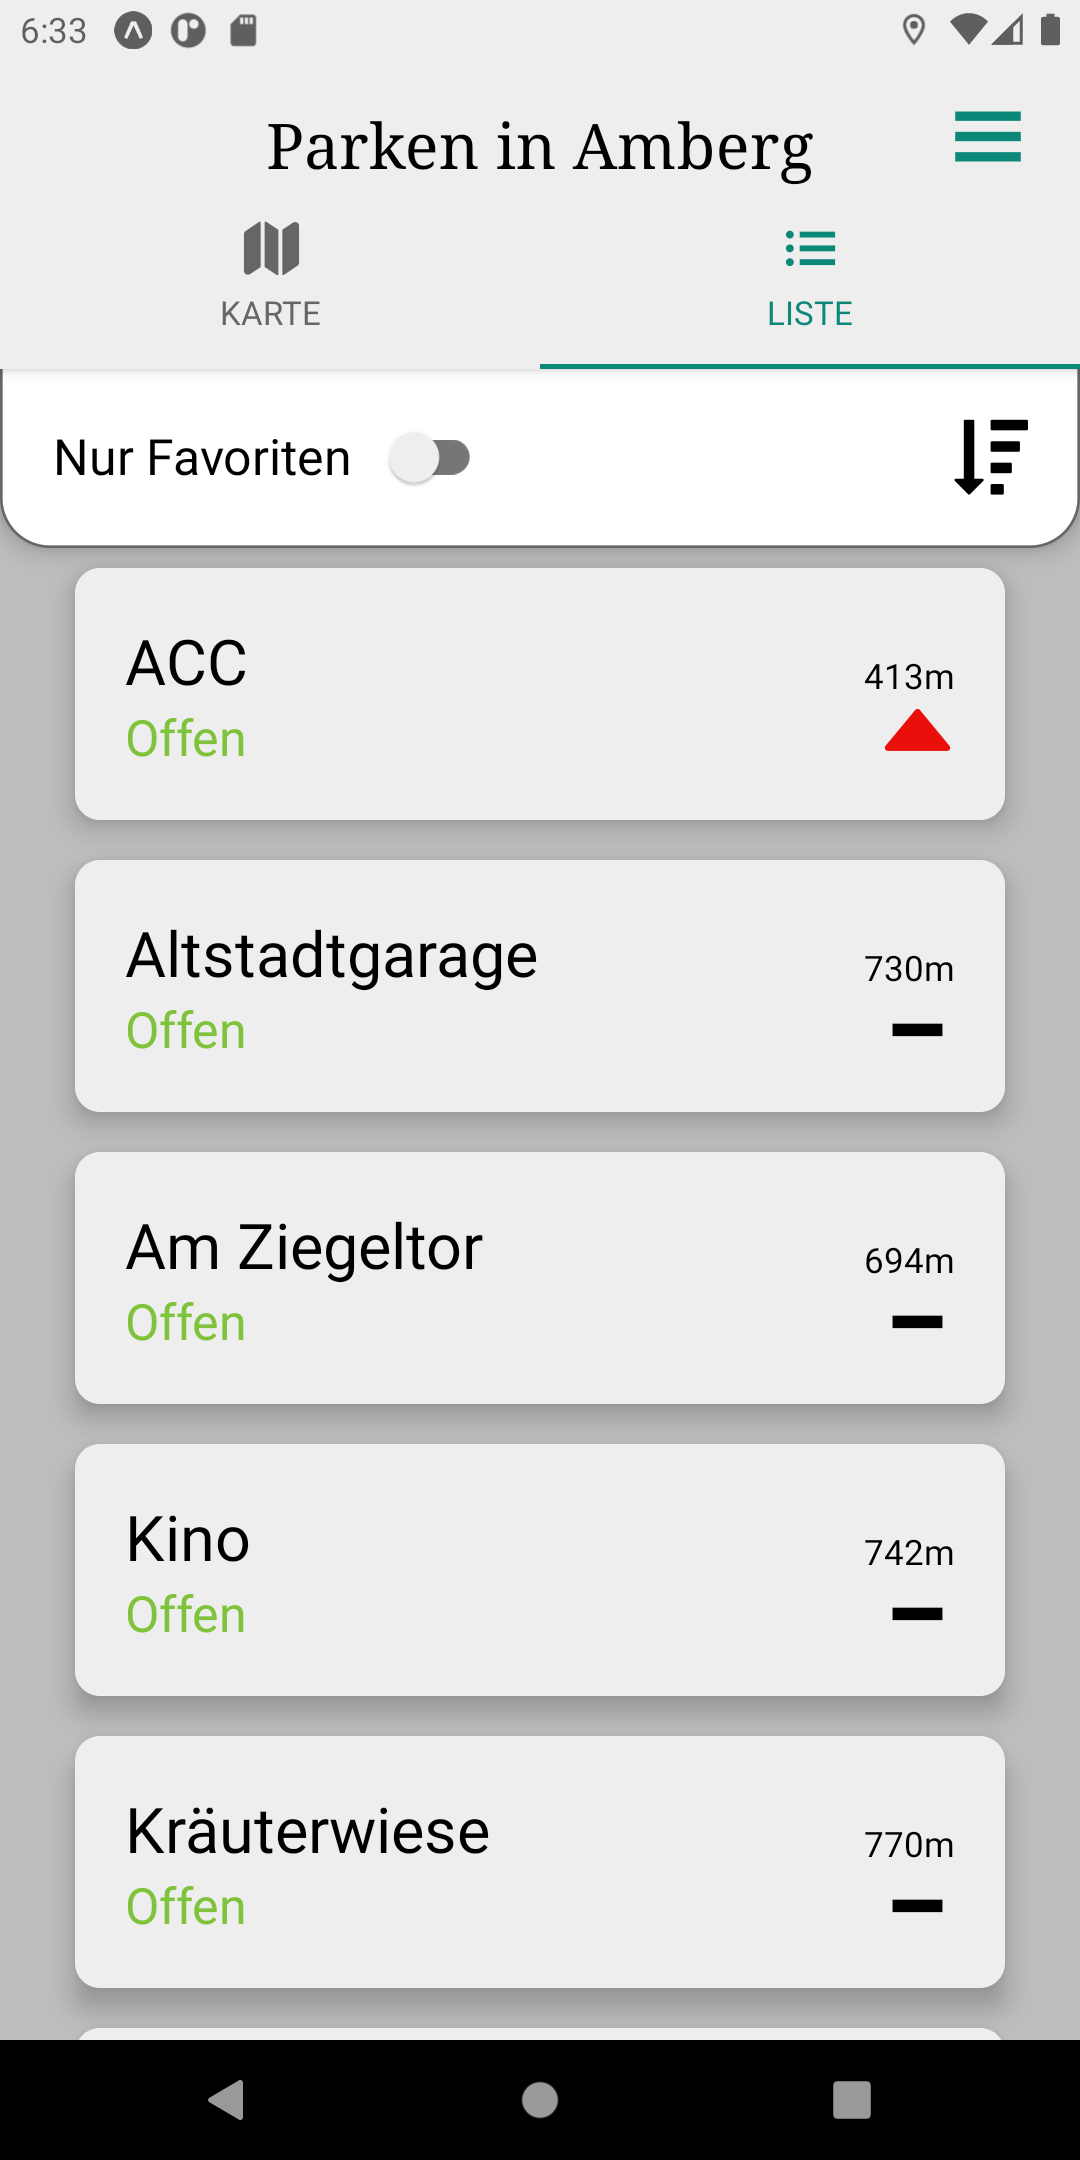
\includegraphics[scale=0.15]{img/list}
	\caption{Ansicht des Listen-Tabs mit der alphabetisch geordneten Liste an Parkhäusern}
	\label{fig:list}
\end{wrapfigure}
Alle Komponenten, aus denen die Liste besteht, sind im Ordner \verb|ParkingList| zu finden. Für die Liste selbst wird die FlatList-Komponente, welche standardmäßig im react-native Framework enthalten ist, verwendet. Dafür wird durch eine Funktion ein Array aus den dynamischen und statischen Daten erzeugt, welche an die FlatList-Komponente zur Anzeige übergeben wird. Die Erzeugung und Anzeige des Arrays ist in der Datei \verb|ParkingList.tsx| zu finden. Die anzuzeigenden Daten sind zum einen der Name des Parkhauses zur Identifizierung. Darunter wird dargestellt, ob das Parkhaus geöffnet oder geschlossen ist. Wenn das Parkhaus offen ist, wird dies in grüner Schrift angezeigt, geschlossen wird dagegen rot geschrieben. Da alle Parkhäuser 24 Stunden offen sind, sollte ein geschlossenes Parkhaus nur bei Wartungsarbeiten und Störungen auftreten. Rechts daneben wird die Entfernung des Nutzers zu diesem spezifischen Parkhaus in Metern angezeigt. Die Position des Nutzers wird wieder über dieselbe Methode erlangt, wie in \autoref{chap:3} für das Geofencing. Über die Haversine Distanz wird wieder die Entfernung zu den Koordinaten der Parkhäuser berechnet und dann angezeigt. Dies wird bei jeder Positionsänderung des Nutzers durchgeführt, damit die Entfernungen immer aktuell sind. Darunter wird noch der Trend des Parkhauses über Icons symbolisiert. Ein grüner Pfeil nach unten signalisiert, dass sich das Parkhaus leert, ein roter Pfeil nach über bedeutet ein sich füllendes Parkhaus und ein schwarzer Balken zeigt einen gleichbleibenden Trend an, wie mit den Markern der Karte.

\begin{wrapfigure}{R}{0.5\textwidth}
	\vspace{-\baselineskip}
	\centering
	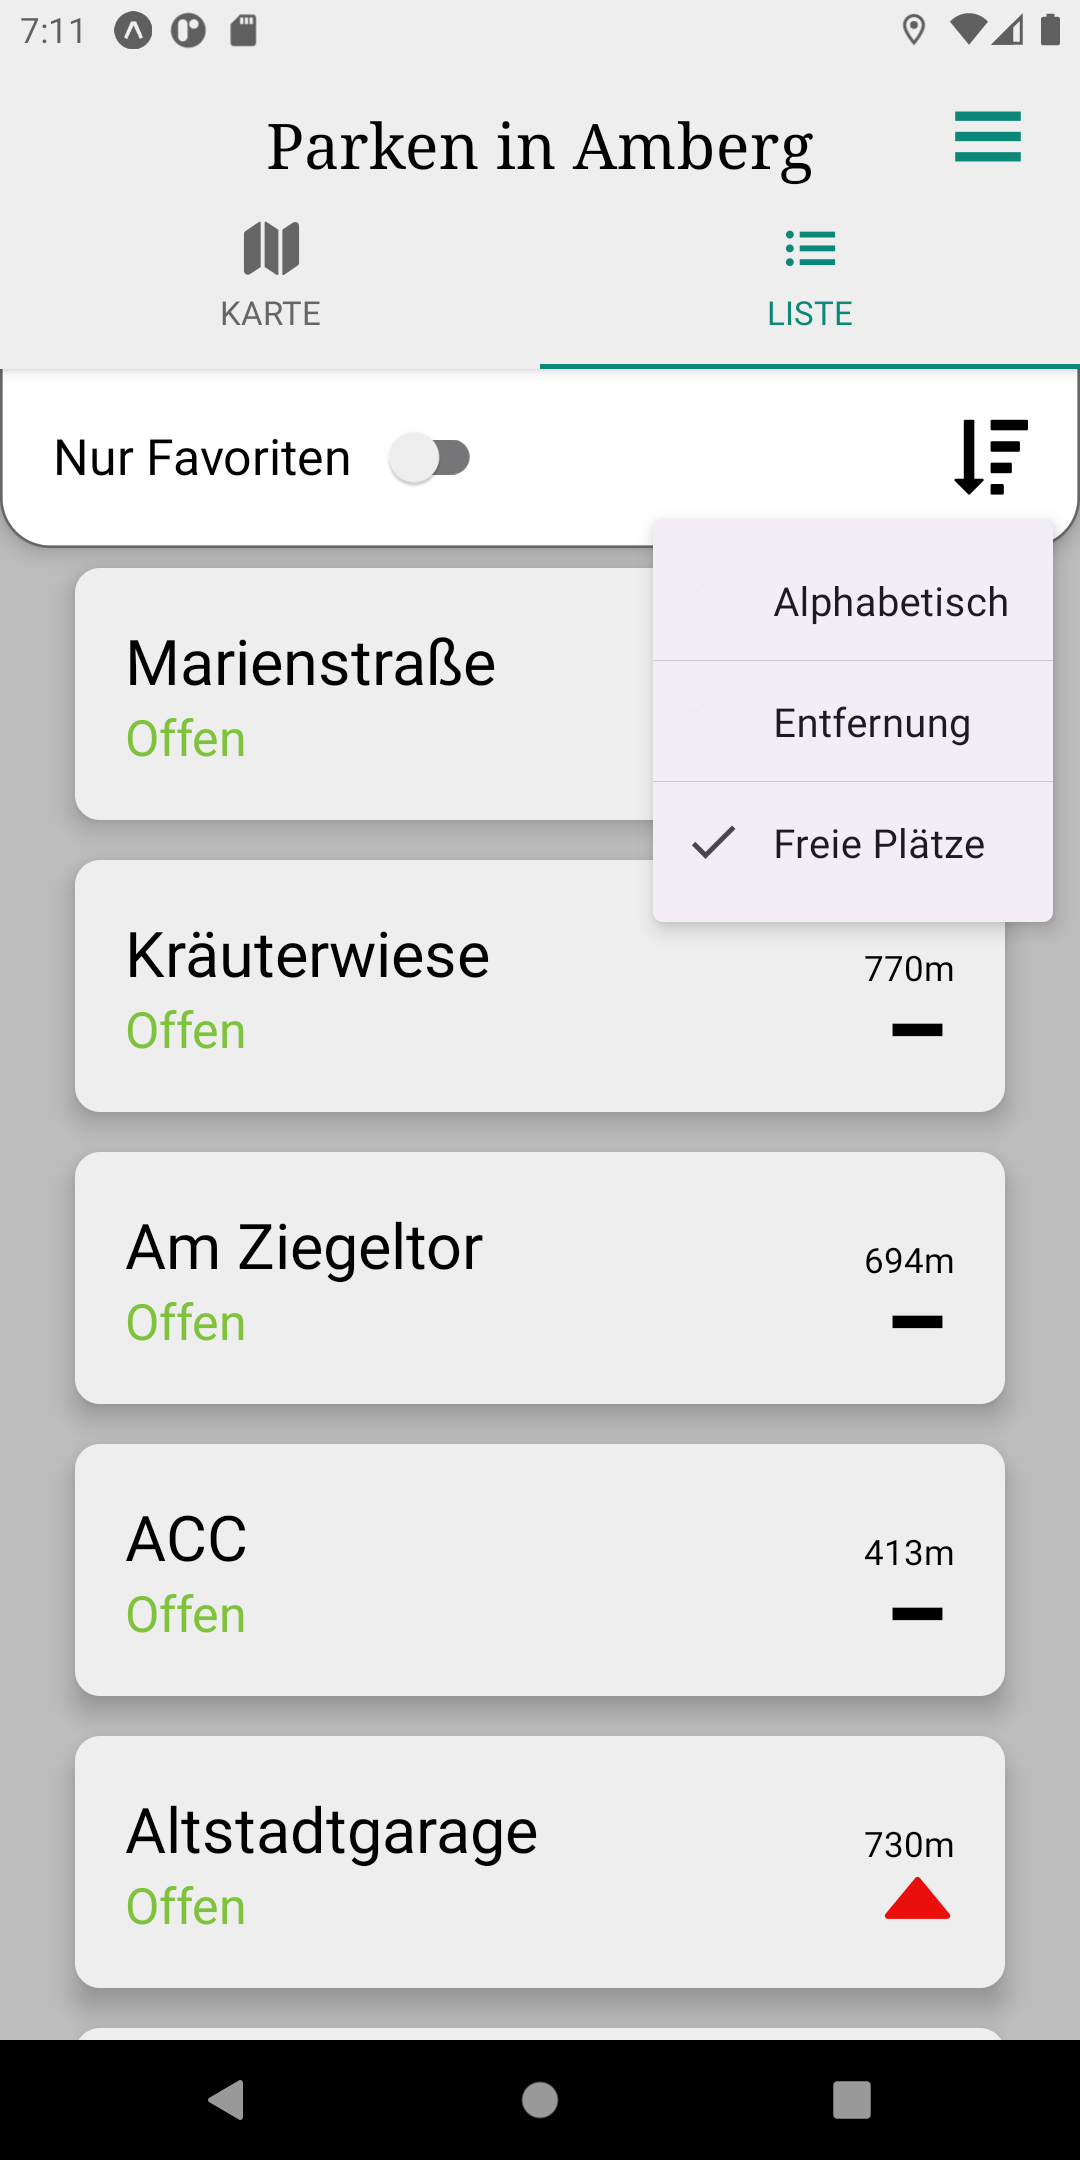
\includegraphics[scale=0.15]{img/sorting}
	\caption{Aufruf des Menüs zum Sortieren der Liste}
	\label{fig:sorting}
\end{wrapfigure}
Diese Liste kann zudem auch konfiguriert werden. Dafür ist zu einen links oben der Liste ein Schalter vorhanden, für den die Switch-Komponente von react-native benutzt wurde, mit der Beschreibung ,,Nur Favoriten''. Wenn dieser Schalter gesetzt ist, werden nur die Parkhäuser angezeigt, welche als Favorit markiert wurden, also bei welchen das rote Herz ausgefüllt ist, wie in \autoref{fig:detail_map} zu sehen ist. Zudem ist rechts oben ein Sortier-Icon zu sehen. Wenn auf dieses Icon geklickt wird öffnet sich eine Liste an Sortiermöglichkeiten, wobei dieses Menü wieder aus dem Paket react-native-paper stammt. Diese Liste ist in \autoref{fig:sorting} ersichtlich. Es gibt drei Sortiermöglichkeiten. Die erste sortiert alphabetisch nach den Namen der Parkhäuser. Die zweite sortiert aufsteigend nach den Entfernungen, sodass das näheste Parkhaus ganz oben steht. Da die Entfernungen bei jeder Positionsänderung des Nutzers neu berechnet werden, muss auch die Liste neu sortiert werden, wenn ein Parkhaus nach einer Positionsänderung näher als ein anderes am Nutzer ist, damit das näheste Parkhaus immer oben ist. Die letzte Möglichkeit sortiert absteigend nach den freien Plätzen, also je mehr Parkplätze in einem Parkhaus frei sind, desto weiter oben ist es in der Liste.

Da es nicht möglich war, alle Daten zu den Parkhäusern in der Liste anzuzeigen, mussten Detail-Fenster erzeugt werden, die nähere Informationen zu den Parkhäusern darstellen. Diese Detail-Fenster sind über Anklicken des zugehörigen Listeneintrags aufrufbar. Um zwischen der Liste und den verschiedenen Detail-Fenstern der Parkhäuser navigieren zu können, wurde das Paket React Navigation benutzt. Dieses ermöglicht das Aufrufen von Fenstern über die Screen-Komponente. Diese Fenster besitzen einen Zurück-Knopf, wie in \autoref{fig:details1} ersichtlich, mit dem zum letzten Fenster, also der Liste, zurück navigiert werden kann. Das Detail-Fenster besitzt zudem auch die Navigations- und Favoriten-Icons der Karte, welche hier dieselbe Funktion besitzen. Durch Drücken des Navigations-Icons wird der Nutzer hier jedoch entweder zur Karte für die interne Navigation, oder direkt zu Google Maps weitergeleitet.

\begin{wrapfigure}{r}{0.5\textwidth}
	\vspace{-\baselineskip}
	\centering
	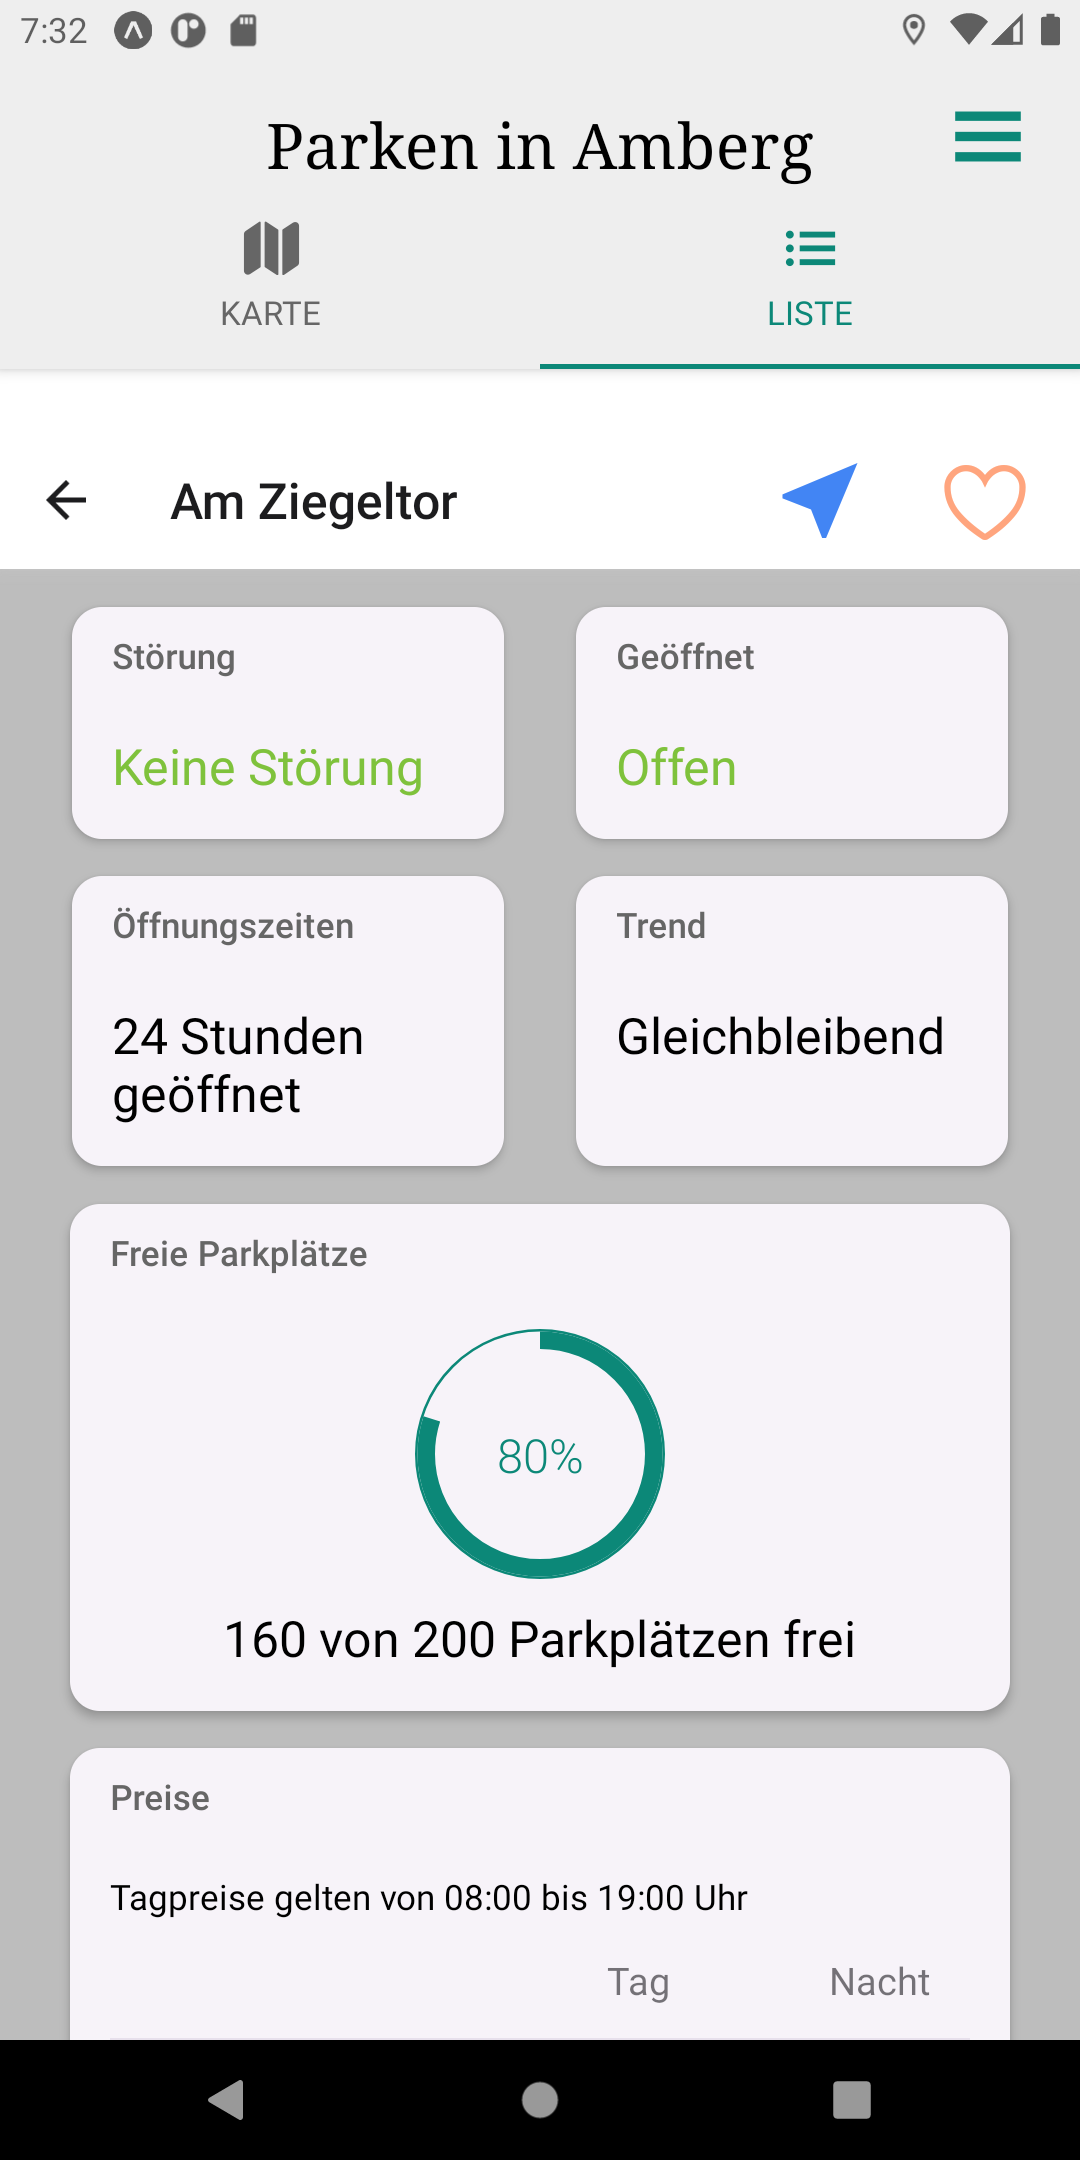
\includegraphics[scale=0.13]{img/details1}
	\caption{Erster Teil des Detail-Fensters zum Parkhaus am Ziegeltor}
	\label{fig:details1}
\end{wrapfigure}
Zur Anzeige der restlichen Informationen des Parkhauses wurde wieder das react-native-paper Paket benutzt. Hier bestehen die weißen Kasten, aus denen sich das Detail-Fenster zusammensetzt, aus der Card Komponente. Zuerst wird durch rote oder grüne Schrift gezeigt, ob es in diesem Parkhaus gerade eine Störung gibt oder nicht und ob das Parkhaus offen ist. Danach werden die Öffnungszeiten angeschrieben und der Trend nochmals schriftlich gezeigt. Darunter wird die Anzahl der freien Parkplätze auf dieselbe Weise wie in der Karte gezeigt.

\begin{wrapfigure}{r}{0.5\textwidth}
	\vspace{-\baselineskip}
	\centering
	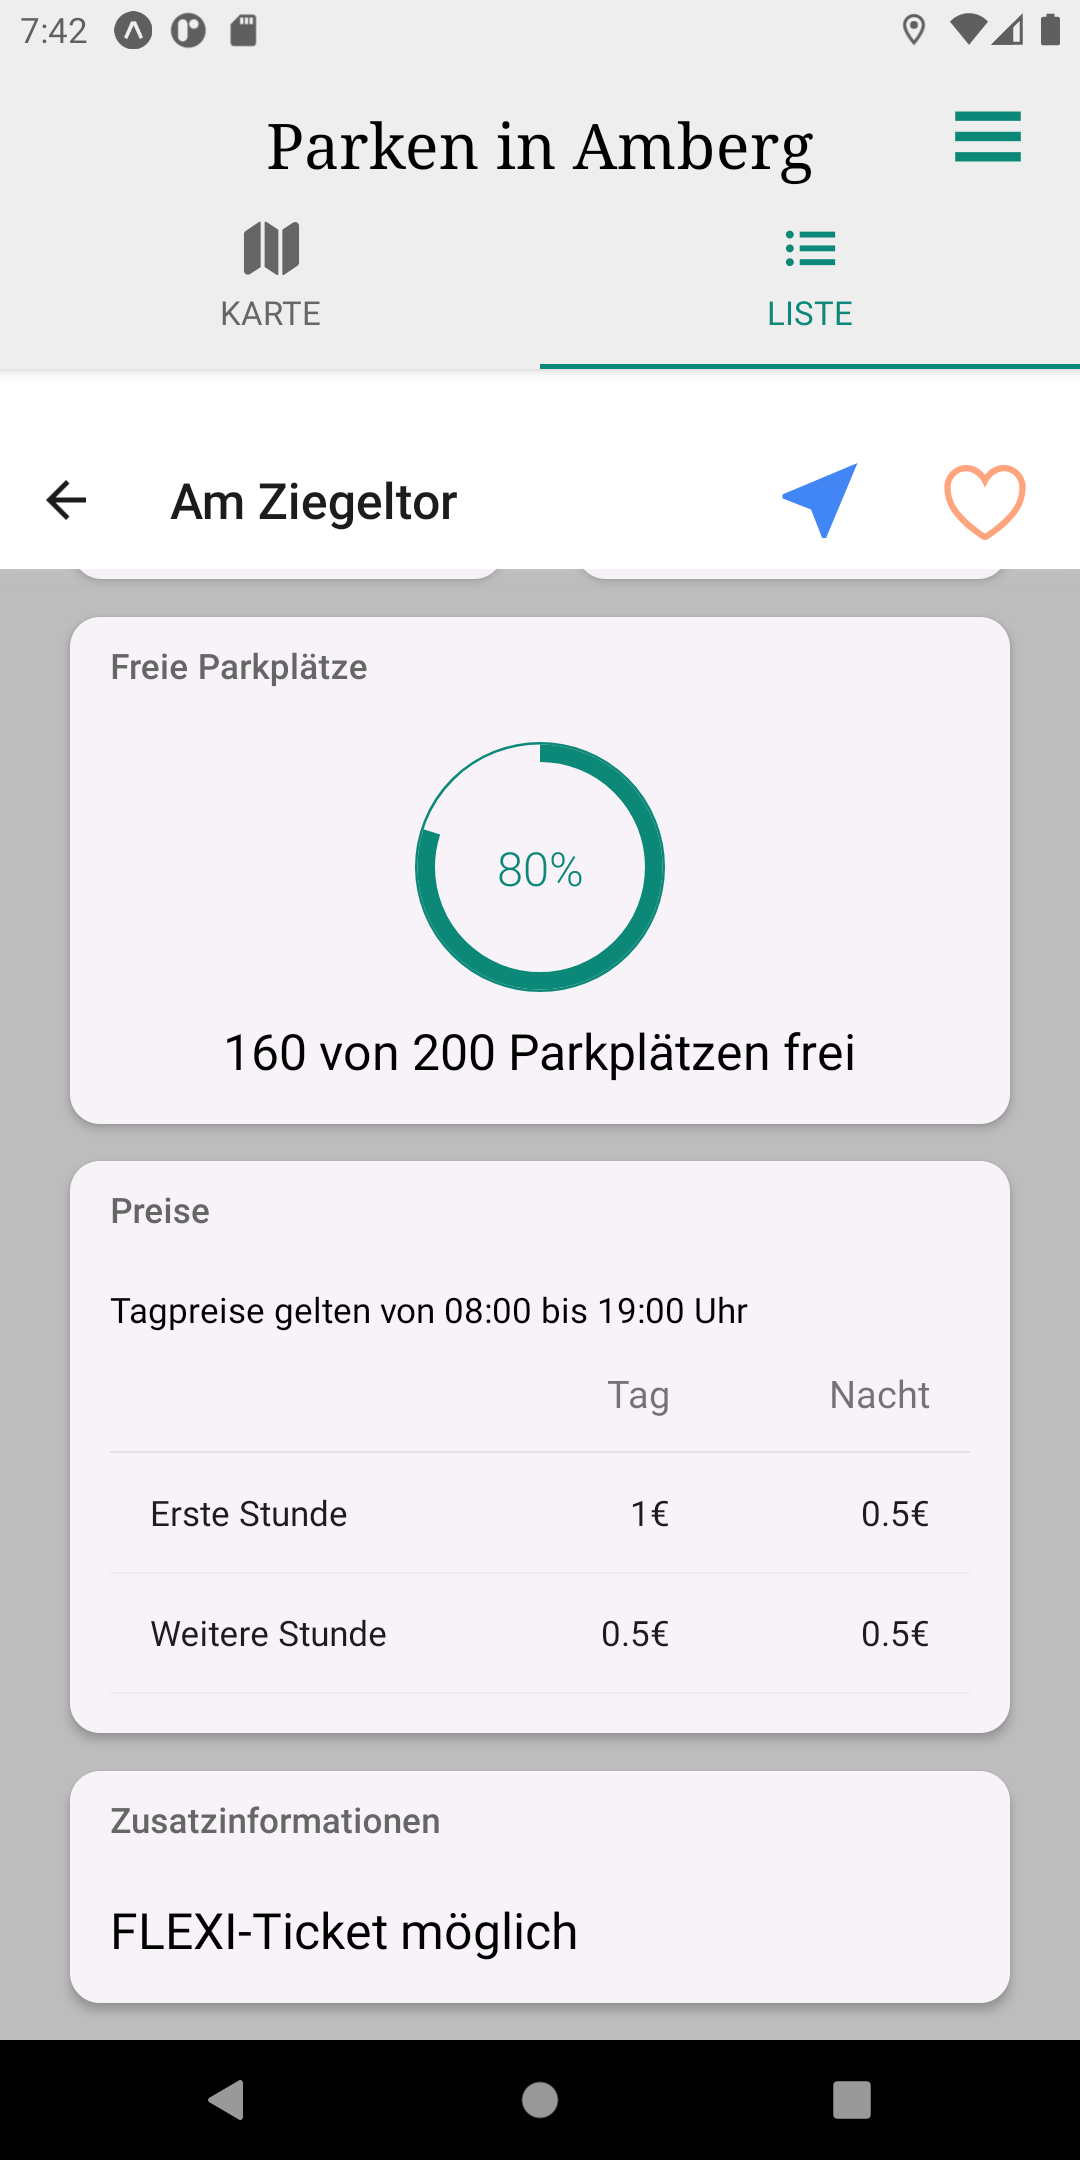
\includegraphics[scale=0.12]{img/details2}
	\caption{Zweiter Teil des Detail-Fensters zum Parkhaus am Ziegeltor}
	\label{fig:details2}
\end{wrapfigure}
Unter den freien Parkplätzen sind die Preise dargestellt. Wenn eine Unterscheidung in Tag- und Nachtpreise nötig ist, wie beim Parkhaus am Ziegeltor, werden diese Preise als Tabelle gezeigt, wobei hier jeweils der Preis für die erste und die weiteren Stunden eingetragen ist. Die Tabelle besteht aus der DataTable-Komponente des react-native-paper Pakets. Unter den Preisen sind nur noch die Zusatzinformationen der statischen Daten zu sehen. Damit werden alle verfügbaren Daten angezeigt und dem Nutzer übersichtlich und benutzerfreundlich dargestellt.

Damit sind alle Komponenten und Funktionalitäten der Liste beschrieben worden. Um die Funktionsweise und den Effekt der Navigationsknöpfe in der Karte und in den Detail-Fenstern der Parkhäuser besser verstehen zu können, wird im nächsten Kapitel auf die interne Pseudo-Navigation eingegangen, welche für diese App erstellt wurde und wie diese Navigation reagiert, wenn kein Weg zum Parkhaus gefunden werden kann.

